\chapter{Penggalian Data}
\label{chap:penggalian data}
Pada bab ini dijelaskan analisis masalah penelitian ini. Analisis meliputi langkah-langkah \textit{query} yang dilakukan dengan data yang lebih besar. \textit{query} yang dilakukan sama dengan bab sebelumnya \ref{langkah_query} tetapi tidak menggunakan \textit{limit}. Pada bab ini juga menampilkan beberapa chart dari apliakasi untuk menunjukkan jumlah pengunaan aplikasi dengan versi yang paling banyak digunakan. ]

\section{Langkah-Langkah \textit{Query} Yang Dilakukan Dengan Data Yang Lebih Besar}
Pada \textit{section} ini dijelaskan tentang langkah-langkah \textit{query} yang dilakukan dalam memperoleh data. Data yang diambil adalah semua data yang didapatkan dengan menggunakan \textit{query}. Data yang diambil merupakan \textit{dataset} dari tabel \textit{technologies} 2020$\_$08$\_$01:

\subsection{Mengumpulkan \textit{List Website}}
Langkah pertama yang dilakukan yaitu mengumpulkan \textit{website}. \textit{Website} yang dicari tidak berdasarkan berdasarkan \textit{rank} karena tidak tersedia pada \textit{dataset} tersebut. \textit{Query} yang digunakan untuk mengumpulkan \textit{list website} dapat dilihat pada Gambar \ref{lst:listwebsite}.
\begin{lstlisting}[caption={Mendapatkan Daftar \textit{Website}}, label={lst:listwebsite}]
SELECT 
	url
FROM 
	`httparchive.technologies.2020_08_01_*`
ORDER BY 
	url ASC
\end{lstlisting}

Pada \textit{query} diatas dilakukan pemilihan pada kolom url dengan menggunakan perintah SELECT dari project httparchive dataset \textit{technologies} tabel 2020\_08\_01\_* dengan menggunakan perintah FROM. Mengelompokan pada kolom url yang dilakukan dengan menggunakan perintah GROUP BY sehingga tidak ada nama url yang sama.  10 contoh halaman awal yang dapat dilihat pada Tabel \ref{table:contoh_langkah411} dan 10 contoh halaman akhir dari hasil keluaran yang dapat dilihat pada Tabel \ref{table:contoh_langkah412} dari \textit{query} diatas:

\begin{table}[H]
	\centering
	\begin{tabular}{|l|l|}
		\hline
		\textbf{Row} & \textbf{url}\\
		\hline
		1 & https://www.theinsider.life/\\
		\hline
		2 & http://www.mtctutorials.com/ \\
		\hline
		3 & https://noticias24horases.com.br/\\
		\hline
		4 & https://www.tonyburke.com.au/ \\
		\hline
		5 & http://www.bakedbyjoanna.com/\\
		\hline
		6 & https://stuftburgerbar.com/\\
		\hline
		7 & https://www.skagitpowersports.com/\\
		\hline
		8 & http://www.arazatimaderas.com/ \\
		\hline
		9 & https://oasisexc.com/\\
		\hline
		10 & https://www.captainslanding.com/\\
		\hline
	\end{tabular}
	\caption{10 Halaman Awal Hasil Pengumpulan Daftar Website}
	\label{table:contoh_langkah411}
\end{table}

\begin{table}[H]
	\centering
	\begin{tabular}{|l|l|}
		\hline
		\textbf{Row} & \textbf{url}\\
		\hline
		7515741 & https://zypa.ru/
		\\
		\hline
		7515742 & https://zyrardow.eglos.pl/
		 \\
		\hline
		7515743 & https://zyrtec.pl/
		\\
		\hline
		7515744 & https://zytecgermbuster.ca/
		 \\
		\hline
		7515745 & https://zythom.blogspot.com/
		\\
		\hline
		7515746 & https://zzso27.wordpress.com/
		\\
		\hline
		7515747 & https://zzslot8.com/
		\\
		\hline
		7515748 & https://zzzttt.me/
		 \\
		\hline
		7515749 & https://zzzzzztema.itch.io/
		\\
		\hline
		7515750 & https://zzzzzzzzz9.pixnet.net/
		\\
		\hline
	\end{tabular}
	\caption{10 Halaman Akhir Hasil Pengumpulan Daftar Website}
	\label{table:contoh_langkah412}
\end{table}

\subsection{Mencari Aplikasi Yang Digunakan \textit{Website}}
Setiap \textit{website} dicari aplikasi apa saja yang digunakan dalam pembangunan \textit{website} tersebut dan versi dari aplikasi yang dipakainya. \textit{Query} yang digunakan dapat dilihat pada Gambar \ref{lst:webapp}.
\begin{lstlisting}[caption={Mencari Aplikasi yang Digunakan Website}, label={lst:webapp}]
SELECT 
	url, app
FROM 
	`httparchive.technologies.2020_08_01_*`
ORDER BY 
	url ASC
\end{lstlisting}

Pada \textit{query} diatas dilakukan pemilihan pada kolom url dan app dengan menggunakan perintah SELECT dari \textit{project} httparchive \textit{dataset} \textit{technologies} tabel 2020\_08\_01\_* dengan menggunakan perintah FROM. Kolom diurutkan berdasarkan url secara \textit{ascending}. 10 contoh halaman awal yang dapat dilihat pada Tabel \ref{table:contoh_langkah421} dan 10 contoh halaman akhir dari hasil keluaran yang dapat dilihat pada Tabel \ref{table:contoh_langkah422} dari \textit{query} diatas:

\begin{table}[H]
	\centering
	\begin{tabular}{|l|l|l|}
		\hline
		\textbf{Row} & \textbf{url} & \textbf{app}\\
		\hline
		1 & http://0-1.ru/ & Liveinternet\\
		\hline
		2 & http://0-1.ru/ & Yandex.Metrika\\
		\hline
		3 & http://0-1.ru/ & IIS\\
		\hline
		4 & http://0-1.ru/ & Microsoft ASP.NET\\
		\hline
		5 & http://0-1.ru/ & YouTube\\
		\hline
		6 & http://0-1.ru/ & Windows Server\\
		\hline
		7 & 	
		http://0-10-10.cocolog-nifty.com/  & 	
		Nginx \\
		\hline
		8 & 	
		http://0-10-10.cocolog-nifty.com/  & Twitter\\
		\hline
		9 & 	
		http://0-10-10.cocolog-nifty.com/  & jQuery\\
		\hline
		10 & 	
		http://0-10-10.cocolog-nifty.com/  & Osano\\
		\hline
	\end{tabular}
	\caption{10 Halaman Awal Contoh Aplikasi Yang Digunakan Website}
	\label{table:contoh_langkah421}
\end{table}

\begin{table}[H]
	\centering
	\begin{tabular}{|l|l|l|}
		\hline
		\textbf{Row} & \textbf{url} & \textbf{app}\\
		\hline
		75873774 & https://zzzzzzzzz9.pixnet.net/
		 & Criteo\\
		\hline
		75873775 &https://zzzzzzzzz9.pixnet.net/
		 & Babel\\
		\hline
		75873776 &https://zzzzzzzzz9.pixnet.net/
		 & YouTube\\
		\hline
		75873777 & https://zzzzzzzzz9.pixnet.net/
		 & SWFObject
		 \\
		\hline
		75873778 & https://zzzzzzzzz9.pixnet.net/
		 & YouTube\\
		\hline
		75873779 & https://zzzzzzzzz9.pixnet.net/
		 & Mixpanel\\
		\hline
		75873780 & 	
		https://zzzzzzzzz9.pixnet.net/
		  & 	
		Google Analytics
		 \\
		\hline
		75873781 & 	
		https://zzzzzzzzz9.pixnet.net/
		  & Google Plus
		  \\
		\hline
		75873782 & 	
		https://zzzzzzzzz9.pixnet.net/
		  & jQuery\\
		\hline
		75873783 & 	
		https://zzzzzzzzz9.pixnet.net/
	  & VideoJS\\
		\hline
	\end{tabular}
	\caption{10 Halaman Akhir Contoh Aplikasi Yang Digunakan Website}
	\label{table:contoh_langkah422}
\end{table}

\subsection{Mengelompokkan Berdasarkan Nama Semua Aplikasi Yang Dipakai}
Pengelompokan aplikasi dapat dilakukan dengan menggunakan \textit{query}. \textit{query} yang digunakan dapat dilihat pada Gambar \ref{lst:groupapp}.
\begin{lstlisting}[caption={Mengelompokan Semua Aplikasi yang Dipakai}, label={lst:groupapp}]
SELECT 
	tabelName.app, num.num_sites , versioned.versioned_count , unversioned.unversioned_count
FROM (
	SELECT DISTINCT 
		app
	FROM 
		`httparchive.technologies.2020_08_01_*` ) tabelName

	LEFT JOIN 

	(
	SELECT 
		tabel1.app, count(app) AS versioned_count
	FROM 
		`httparchive.technologies.2020_08_01_*` AS tabel1
	WHERE 
		tabel1.app!="" AND tabel1.info != "" 
	GROUP BY 
		tabel1.app) AS versioned

	ON(versioned.app = tabelName.app)

	LEFT JOIN

	(
	SELECT 
		tabel2.app, count(app) AS unversioned_count
	FROM 
		`httparchive.technologies.2020_08_01_*` AS tabel2
	WHERE 
		tabel2.app!="" AND tabel2.info = "" 
	GROUP BY 
		tabel2.app) AS unversioned

	ON (unversioned.app = tabelName.app)

	LEFT JOIN 

	(
	SELECT 
		app, count(url) AS num_sites
	FROM 
		`httparchive.technologies.2020_08_01_*`
	GROUP BY 
		app) AS num

	ON (tabelName.app = num.app)
\end{lstlisting}

Pada \textit{query} diatas dibuat beberapa tabel baru yang bersifat sementara. Pada baris ke 3 dan 4, \textit{query} mengembalikan tabel yang berisi semua app yang ada pada tabel menggunakan perintah SELECT dan menggunakan DISTINCT agar app yang ditampilkan hanya keluar satu kali. Data diambil dari \textit{project} httparchive \textit{dataset} \textit{technologies} tabel 2020\_08\_01\_* dengan menggunakan perintah FROM. Kemudian pada baris ke 8 sampai 11, \textit{query} mengembalikan tabel yang berisi app dan jumlah app yang memiliki info tidak kosong atau memiliki informasi versi. Pada baris 17 sampai 22, \textit{query} mengembalikan tabel yang berisi app dan jumlah app yang tidak memiliki informasi versi. Pada baris 26 sampai dengan baris 28, \textit{query} mengembalikan tabel app, jumlah url yang menggunakan app tersebut. Kemudian semua tabel tersebut digabungkan dengan perintah LEFT JOIN. Kemudian dengan menggunakan perintah SELECT, dipanggil beberapa variabel dari setiap kolom dari setiap tabel. Kolom yang diambil berupa: app, jumlah situs yang dipakai aplikasi (num\_sites), jumlah aplikasi yang memiliki versi (versioned\_count), dan jumlah aplikasi yang tidak memiliki versi (unversioned\_count). 10 contoh halaman awal yang dapat dilihat pada Tabel \ref{table:contoh_langkah431} dan 10 contoh halaman akhir dari hasil keluaran yang dapat dilihat pada Tabel \ref{table:contoh_langkah432} dari \textit{query} diatas:

\begin{table}[H]
	\centering
	\begin{tabular}{|l|l|r|r|r|}
		\hline
		\textbf{Row} & \textbf{app} & \textbf{num\_sites} & \textbf{versioned\_count} & \textbf{unversioned\_count}\\
		\hline
		1 & jQuery & 10.003.030 & 9.979.001 & 24.029\\
		\hline
		2 & Apache & 4.067.380 & 1.118.200 & 2.949.180\\
		\hline
		3 & PHP & 5.977.790 & 2.522.620 & 3.455.170\\
		\hline
		4 & MySQL & 4.047.343 & null & 4.047.343\\
		\hline
		5 & Microsoft SharePoint & 14.419 & 11.402 & 3.017\\
		\hline
		6 & YouTube & 1.028.360& null & 1.028.360\\
		\hline
		7 & Microsoft ASP.NET & 865.276 & 407.366 & 457.910\\
		\hline
		8 & Google Code Prettify & 32.171 & null & 32.171\\
		\hline
		9 & Typekit & 253.890 & 253.203 & 687\\
		\hline
		10 & Slick & 759.805 & 66.249 & 693.556\\
		\hline
	\end{tabular}
	\caption{10 Halaman Awal Hasil Pengelompokan Aplikasi Beserta Jumlah \textit{Versioned} Dan \textit{Unversioned}}
	\label{table:contoh_langkah431}
\end{table}

\begin{table}[H]
	\centering
	\begin{tabular}{|l|l|r|r|r|}
		\hline
		\textbf{Row} & \textbf{app} & \textbf{num\_sites} & \textbf{versioned\_count} & \textbf{unversioned\_count}\\
		\hline
		1327 & Raphael & 2 & null & 2\\
		\hline
		1328 & Avangate & 2 & null & 2\\
		\hline
		1329 & GoAhead
		 & 3 & null & 3\\
		\hline
		1330 & Banshee & 2 & null & 2\\
		\hline
		1331 & Veoxa & 7 & null & 7\\
		\hline
		1332 & jQuery Sparkline
		 & 2& null & 2\\
		\hline
		1333 &animate.cs
		 & 1 & null & 1\\
		\hline
		1334 & jQuery U
		 & 1 & null & 1\\
		\hline
		1335 & Pars Elecom Portal
		 & 1 & null & 1\\
		\hline
		1336 & Highchart
		 & 1 & null & 1\\
		\hline
	\end{tabular}
	\caption{10 Halaman Akhir Hasil Pengelompokan Aplikasi Beserta Jumlah \textit{Versioned} Dan \textit{Unversioned}}
	\label{table:contoh_langkah432}
\end{table}

\subsection{Mencari Data Tentang Versi Aplikasi Yang Masih Didukung}
Sebelum menentukan suatu aplikasi usang atau tidak, kita harus mencari versi dari setiap aplikasi secara manual. Versi setiap aplikasi dapat dilihat di-\textit{official documentation} dari setiap aplikasi. Hasil pencarian dari aplikasi yang masih didukung dapat dilihat pada Gambar \ref{lamp:A}. 

\subsection{Melakukan Perbandingan Antara Versi Aplikasi Yang Masih Dipakai Sekarang Dengan Versi Aplikasi Yang Masih Didukung}
Setelah mendapatkan data versi minimal dari setiap aplikasi, data tersebut dibandingkan dengan versi aplikasi yang dipakai \textit{url}. \textit{supported} adalah versi aplikasi dari yang dipakai url masih mendukung atau diatas atau sama dengan versi yang didukung didokumen. \textit{unsupported} adalah versi aplikasi dari yang dipakai url sudah tidak mendukung atau dibawah versi yang didukung didokumen. \textit{not\_versioned} adalah versi aplikasi dari url tidak ditampilkan. \textit{non\_conclusive} adalah versi aplikasi tidak dapat ditentukan. Data diambil berdasarkan banyak aplikasi yang dipakai oleh url tertentu. Data yang sudah dibandingkan juga digunakan untuk mencari jumlah \textit{website} yang jumlah semua aplikasinya yang masih didukung. Terdapat 4.280 jumlah aplikasi yang digunakan \textit{website}. \textit{Query} yang digunakan untuk mencari datanya dapat diliha pada Gambar \ref{lst:finalresult}:

\begin{lstlisting}[label={lst:finalresult}, caption={Jumlah \textit{Website} yang Jumlah Semua Aplikasi \textit{Supported} }]
SELECT 
	count(url1.url) as jumlah
FROM 
(
SELECT 
	url, count(app) AS jumlah1
FROM 
	`httparchive-bigquery-346414.app_result.app_result`
WHERE 
	result = "SUPPORTED"
GROUP BY 
	url
ORDER BY 
	url ASC
) AS url1

JOIN 

(
SELECT 
	url, count(app) AS jumlah2
FROM 
	`httparchive-bigquery-346414.app_result.app_result`
GROUP BY 
	url
ORDER BY 
	url ASC
) AS url2

ON url1.url = url2.url
WHERE 
	url1.jumlah1  = url2.jumlah2 
\end{lstlisting}
\textit{Project} httparchive-bigquery-346414 dengan nama \textit{dataset} app\_result dan tabel app\_result adalah sebuah tabel pembantu. Tabel ini berasal dari hasil \textit{version compare} pada \ref{version_compare}. \textit{Project} httparchive-bigquery-346414 ini dibuat berdasarkan data dari \textit{project} httparchive, \textit{dataset} \textit{technologies}, dan tabel 2020\_08\_01\_* yang kemudian dibuat tabel baru agar \textit{query} tidak dipanggil beberapa kali. \\
Pada \textit{query} diatas awalnya dibuat sebuah tabel yang bersifat sementara. Tabel diambil dari  \textit{project} httparchive-bigquery-346414 dengan nama \textit{dataset} app$\_$result dan tabel app$\_$result. Pada tabel ini dicari url dan data dengan informasi versi dari aplikasi yang masih didukung url tersebut, tabel diberi nama url1. Kemudian tabel digabungkan dengan tabel lain yang bersifat sementara. Pada tabel ini dicari semua url dan jumlah aplikasi yang dipakai oleh url tersebut, tabel diberi nama url2. Hasil akhir dari \textit{query} ini berupa url yang dan jumlah dari tabel url1 dan tabel url2. Hasil dari \textit{query} dapat dilihat pada Tabel \ref{table:contoh_langkah451}
\begin{table}[H]
	\centering
	\begin{tabular}{|l|r|}
		\hline
		\textbf{Row} & jumlah\\
		\hline
		1 & 4.280\\
		\hline
	\end{tabular}
	\caption{Jumlah \textit{Website} yang Jumlah Semua Aplikasi \textit{Supported}}
	\label{table:contoh_langkah451}
\end{table}


\section{Hasil Sample Data}
Data yang ditampilkan adalah data beberapa aplikasi yang sudah dipisahkan berdasarkan aplikasi dan nomor versi dari aplikasi yang dipakai serta jumlahnya dalam bentuk \textit{chart}.

\subsection{Apache dan Nginx}
Apache dan Nginx merupakan dua web servers yang paling banyak digunakan. Pada dua web server ini, aplikasi Apache memiliki lebih banyak jumlah yang supported daripada aplikasi Nginx. Pada aplikasi Nginx terdapat 5.440.268 aplikasi yang \textit{unversioned}. Versi pada aplikasi Nginx yang paling banyak digunakan adalah versi 1.14 dengan jumlah 267.102. Pada aplikasi Apache terdapat 2.949.180 aplikasi yang \textit{unversioned}. Versi pada aplikasi Apache yang paling banyak digunakan adalah versi 2.4 dengan jumlah 154.533. Berikut ini adalah chart yang dapat dilihat pada Gambar \ref{fig:data_sample_nginx} dan Gambar \ref{fig:data_sample_apache}:
\begin{figure}[H]
	\centering  
	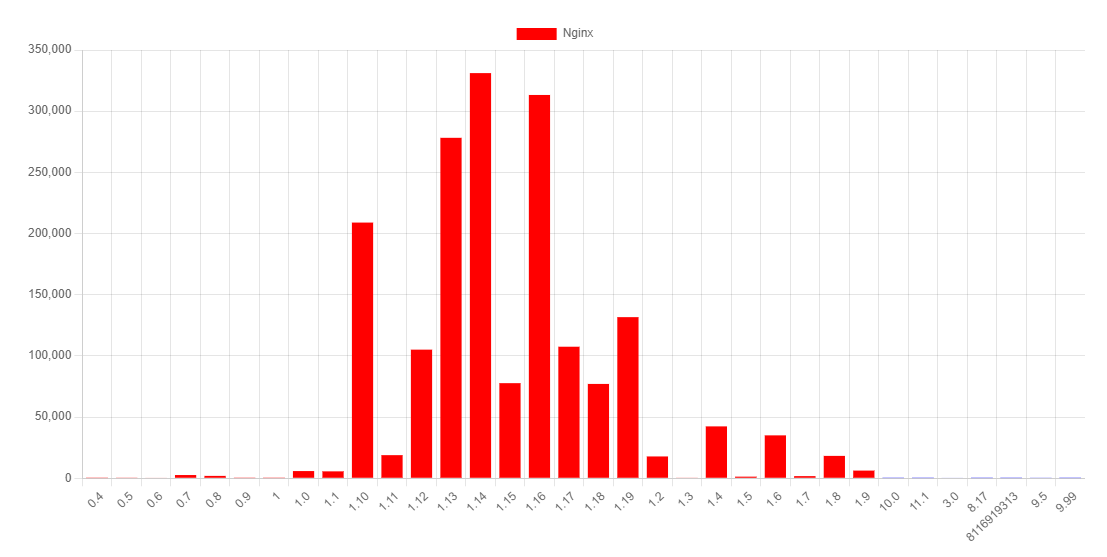
\includegraphics[scale=0.7]{Gambar/data_sample_nginx.png}  
	\caption{Aplikasi Nginx} 
	\label{fig:data_sample_nginx} 
\end{figure}

\begin{figure}[H]
	\centering  
	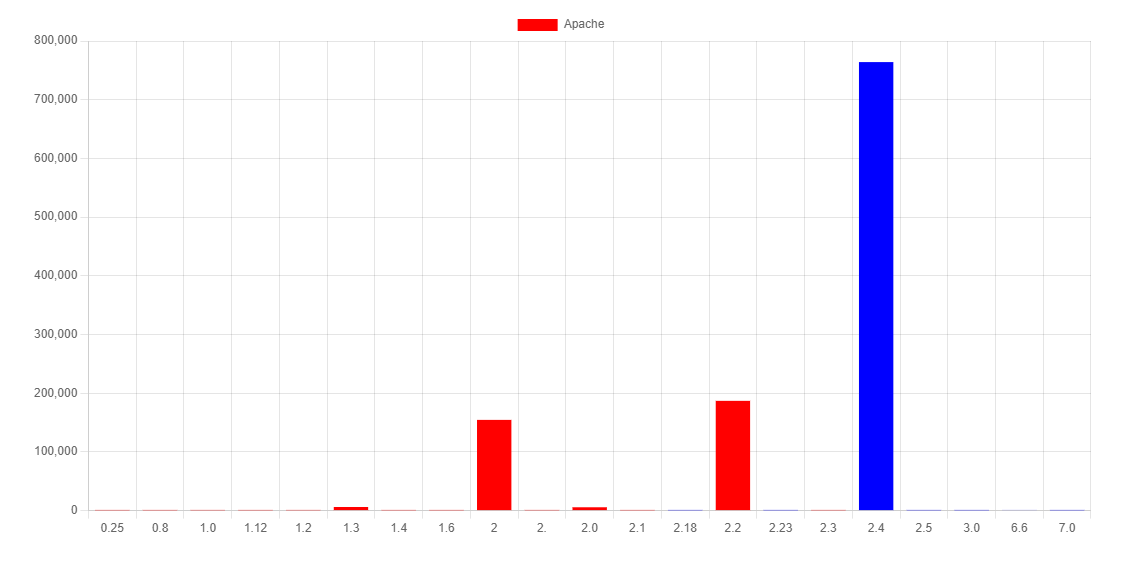
\includegraphics[scale=0.7]{Gambar/apache.png}  
	\caption{Aplikasi Apache} 
	\label{fig:data_sample_apache} 
\end{figure}

Berdasarkan penelitian dengan aplikasi yang sama, didapatkan hasil dalam bentuk \textit{chart}. \textit{Chart} yang dibandingkan dapat dilihat pada Gambar \ref{fig:data_sample_apache_p} dan Gambar \ref{fig:data_sample_nginx_p}.
\begin{figure}[H]
	\centering  
	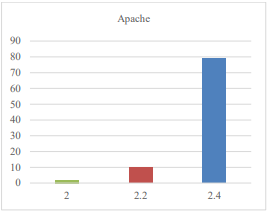
\includegraphics[scale=0.8]{Gambar/chart_pascal_apache.PNG}  
	\caption{Aplikasi Apache dari \cite{pascal}} 
	\label{fig:data_sample_apache_p} 
\end{figure}
\begin{figure}[H]
	\centering  
	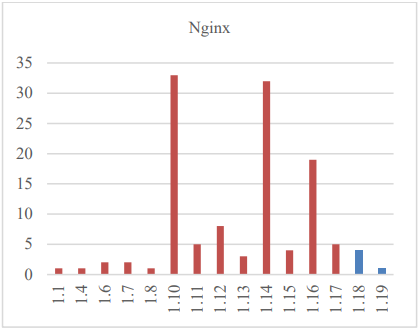
\includegraphics[scale=0.7]{Gambar/chart_pascal_nginx.PNG}  
	\caption{Aplikasi Nginx dari \cite{pascal}} 
	\label{fig:data_sample_nginx_p} 
\end{figure}

\subsection{PHP dan Python}
PHP merupakan bahasa pemograman yang digunakan dalam pembuatan \textit{website}. PHP manjadi bahasa pemograman yang paling banyak digunakan. Pada aplikasi PHP terdapat 3.455.170 aplikasi yang \textit{unversioned}. Versi pada aplikasi PHP yang paling banyak digunakan adalah versi 5.6 dengan jumlah 358.750.
Python merupakan bahasa pemograman tingkat tinggi dan berorientasi objek. Python adalah bahasa pemograman tingkat tinggi karena perintah atau kode program yang digunakan sudah mirip dengan bahasa manusia. Pada aplikasi Python terdapat 360.531 aplikasi yang \textit{unversioned}. Versi pada aplikasi Python yang paling banyak digunakan adalah versi 2.7 dengan jumlah 7.481. Berikut ini adalah \textit{chart} yang dapat dilihat pada Gambar \ref{fig:data_sample_php} dan Gambar \ref{fig:data_sample_python}:
\begin{figure}[H]
	\centering  
	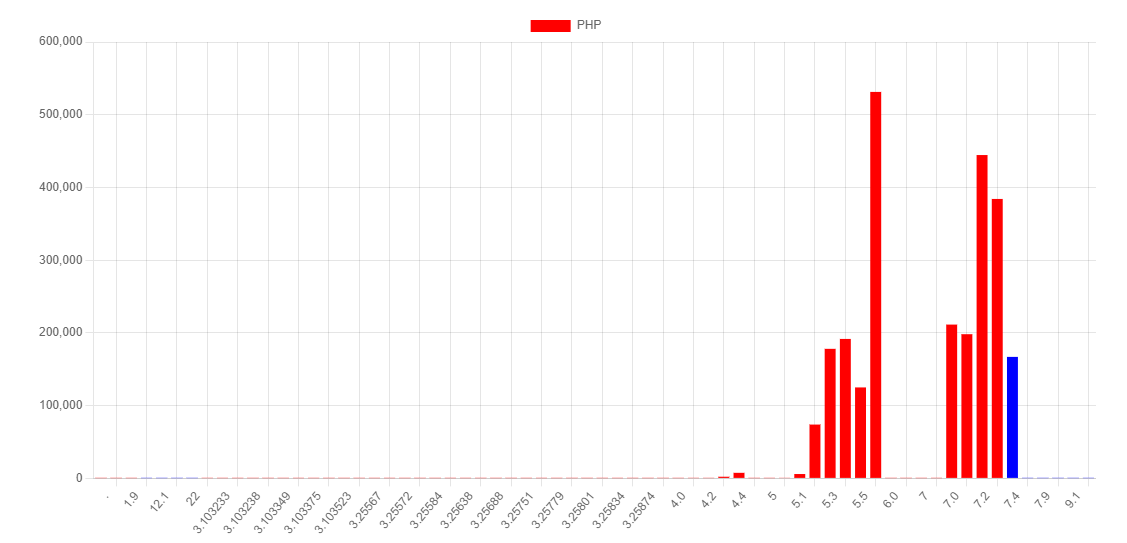
\includegraphics[scale=0.7]{Gambar/data_sample_php.png}  
	\caption{Aplikasi PHP} 
	\label{fig:data_sample_php} 
\end{figure}

\begin{figure}[H]
	\centering  
	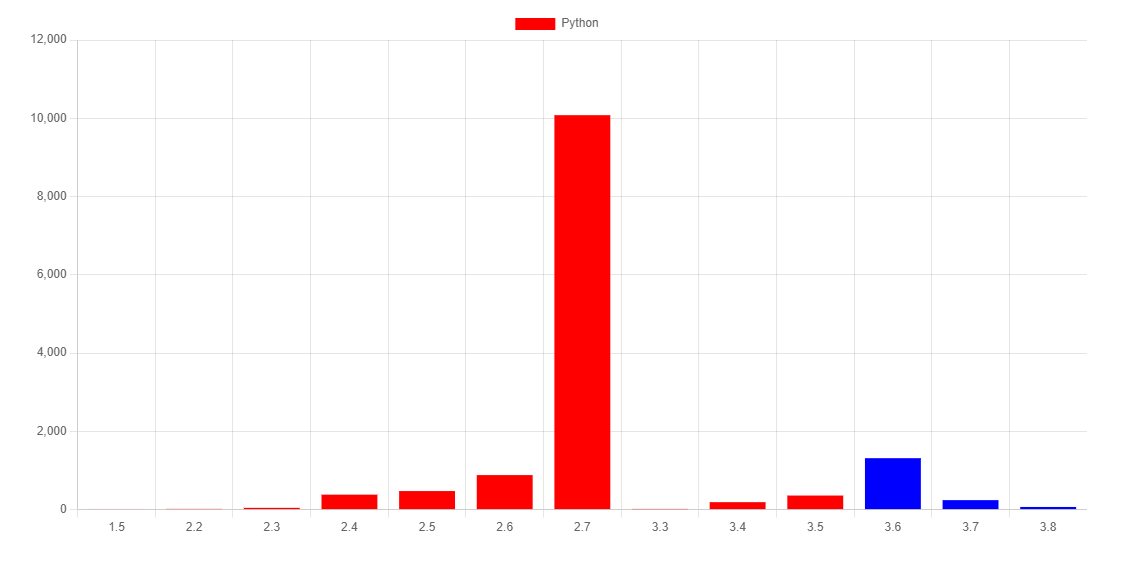
\includegraphics[scale=0.7]{Gambar/data_sample_python.png}  
	\caption{Aplikasi Python} 
	\label{fig:data_sample_python} 
\end{figure}

Berdasarkan penelitian dengan aplikasi yang sama, didapatkan hasil dalam bentuk \textit{chart}. \textit{Chart} yang dibandingkan dapat dilihat pada gambar \ref{fig:data_sample_php_p}.

\begin{figure}[H]
	\centering  
	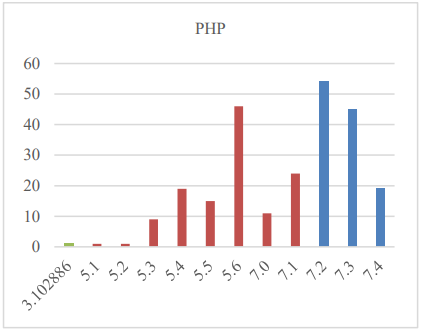
\includegraphics[scale=0.7]{Gambar/chart_pascal_php.PNG}  
	\caption{Aplikasi PHP dari \cite{pascal}} 
	\label{fig:data_sample_php_p} 
\end{figure}

\subsection{jQuery dan jQuery Migrate}
jQuery dan jQuery Migrate merupakan \textit{javascipt libraries} yang paling banyak digunakan. jQuery berfungsi untuk membantu mengatur interaksi antara javascript dan html pada sisi \textit{client}. Pada aplikasi jQuery terdapat 24.029 aplikasi yang \textit{unversioned}. Versi pada aplikasi jQuery yang paling banyak digunakan adalah versi 1.12 dengan jumlah 3.603.522. jQuery Migrate berfungsi untuk membantu memulihkan API yang telah dihapus dan menunjukkan peringatan pada \textit{browser concole}. Pada aplikasi jQuery Migrate terdapat 268.962 aplikasi yang \textit{unversioned}. Versi pada aplikasi jQuery Migrate yang paling banyak digunakan adalah versi 1.4 dengan jumlah 2.935.408. Hasil \textit{chart} dapat dilihat pada Gambar \ref{fig:data_sample_jQuery} dan Gambar \ref{fig:data_sample_jQuery_migrate}
\begin{figure}[H]
	\centering  
	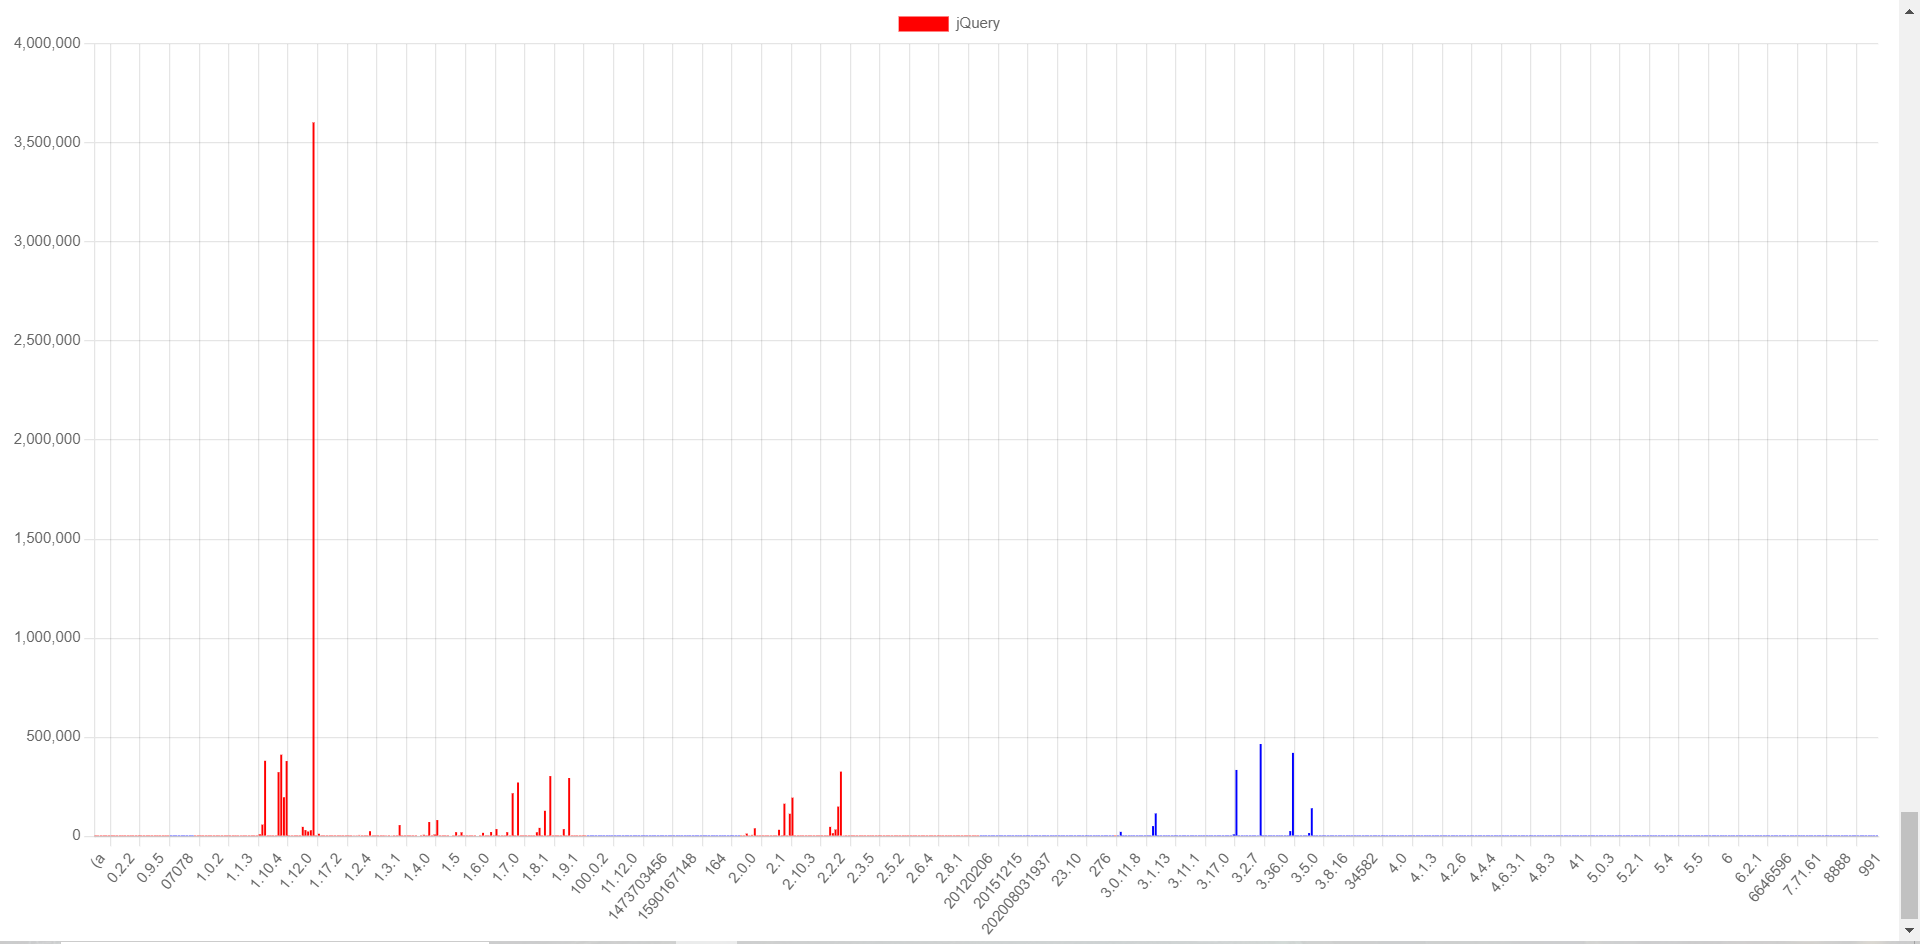
\includegraphics[scale=0.7]{Gambar/data_sample_jQuery.png}  
	\caption{Aplikasi jQuery} 
	\label{fig:data_sample_jQuery} 
\end{figure}

\begin{figure}[H]
	\centering  
	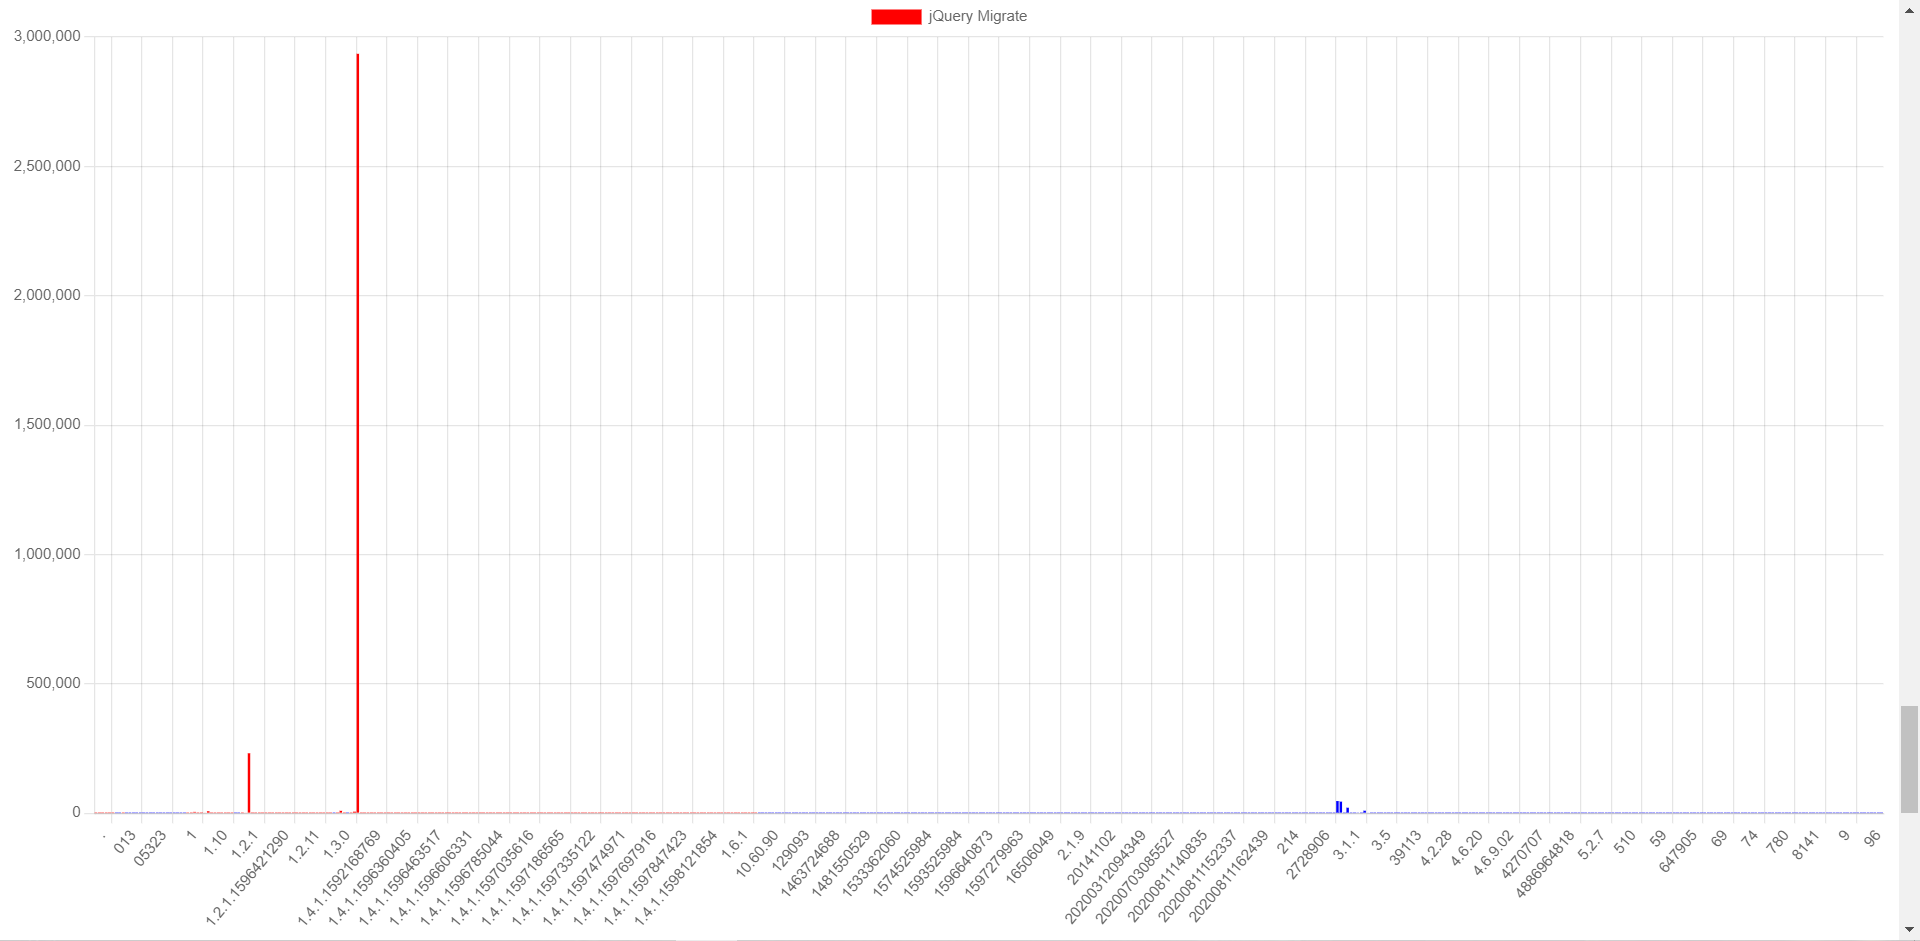
\includegraphics[scale=0.7]{Gambar/data_sample_jQuery_migrate.png}  
	\caption{Aplikasi jQuery Migrate} 
	\label{fig:data_sample_jQuery_migrate} 
\end{figure}

Berdasarkan penelitian dengan aplikasi yang sama, didapatkan hasil dalam bentuk \textit{chart}. \textit{Chart} yang dibandingkan dapat dilihat pada Gambar \ref{fig:data_sample_jQuery_p}.

\begin{figure}[H]
	\centering  
	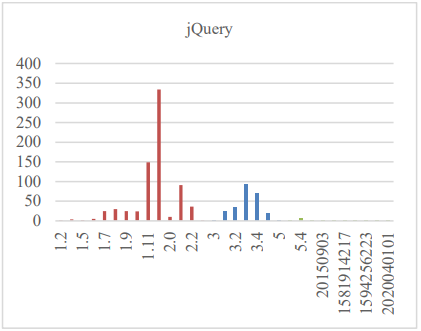
\includegraphics[scale=0.7]{Gambar/chart_pascal_jQuery.PNG}  
	\caption{Aplikasi jQuery dari \cite{pascal}} 
	\label{fig:data_sample_jQuery_p} 
\end{figure}